\clearpage

\titleformat{\section}
  {\normalfont\large\bfseries}{Appendix \thesection}{1em}{}

%% reset figure counter
%% https://tex.stackexchange.com/questions/85776/change-figure-numbering-for-appendix
\renewcommand\thefigure{A\arabic{figure}} 
\setcounter{figure}{0} 

\begin{appendices}

\section{Baseline details and sources}
\label{app:baselines}
\label{app:multitask}

In this section, we provide details about baselines we ran ourselves.
For scores of baselines previously evaluated on standardized tasks, we provide the source of the listed score.

\subsection{Maze2D experiments}
        
\paragraph{Single-task.}

The performance of CQL and IQL on the standard Maze2D environments is reported in the D4RL whitepaper \citep{fu2020d4rl} in Table~2.

We ran IQL using the offical implementation from the authors: 
\begin{center}
{
    \small
    \href{https://github.com/ikostrikov/implicit_q_learning}
    {\texttt{github.com/ikostrikov/implicit\_q\_learning}}.
}
\end{center}

We tuned over two hyperparameters:
\begin{enumerate}
    \item temperature $\in [3, 10]$
    \item expectile $\in [0.65, 0.95]$
\end{enumerate}

\paragraph{Multi-task.}

We only evaluated IQL on the Multi2D environments because it is the strongest baseline in the single-task Maze2D environments by a sizeable margin.
To adapt IQL to the multi-task setting, we modified the $Q$-functions, value function, and policy to be goal-conditioned.
To select goals during training, we employed a strategy based on hindsight experience replay, in which we sampled a goal from among those states encountered in the future of a trajectory.
For a training backup $(\st, \at, \stp)$, we sampled goals according to a geometric distribution over the future
\[
\Delta \sim \text{Geom}(1-\gamma) ~~~~~~~~ \mathbf{g} = \bs_{t + \Delta},
\]
recalculated rewards based on the sampled goal, and conditioned all relevant models on the goal during updating.
During testing, we conditioned the policy on the ground-truth goal.

We tuned over the same IQL parameters as in the single-task setting.

\subsection{Block stacking experiments}

\paragraph{Single-task.}
% BCQ, IQL

We ran CQL using the following implementation
\begin{center}
{
    \small
    \href{https://github.com/young-geng/cql}
    {\texttt{https://github.com/young-geng/cql}}.
}
\end{center}
and used default hyperparameters in the code.
We ran BCQ using the author's original implementation
\begin{center}
{
    \small
    \href{https://github.com/sfujim/BCQ}
    {\texttt{https://github.com/sfujim/BCQ}}.
}
\end{center}

For BCQ, we tuned over two hyperparameters:
\begin{enumerate}
    \item discount factor $\in [0.9, 0.999]$
    \item tau $\in [0.001, 0.01]$
\end{enumerate}

\paragraph{Multi-task.}

To evaluate BCQ and  CQL in the multi-task setting, we modified the $Q$-functions, value function and policy to be goal-conditioned.
We trained using goal relabeling as in the Multi2D environments.
We tuned over the same hyperparameters described in the single-task block stacking experiments.
% BCQ, IQL

% Single-task IQL for maze2d experiments

% Multi-task IQL with hindsight relabeling

% BCQ and IQL for block stacking

\subsection{Offline Locomotion}
\label{app:d4rl_sources}

The scores for BC, CQL, IQL, and AWAC are from Table~1 in \citet{kostrikov2021implicit}.
The scores for DT are from Table~2 in \citet{chen2021decision}.
The scores for TT are from Table~1 in \citet{janner2021sequence}.
The scores for MOReL are from Table~2 in \citet{kidambi2020morel}.
The scores for MBOP are from Table~1 in \citet{argenson2020model}.



\begin{figure}[t]
\centering
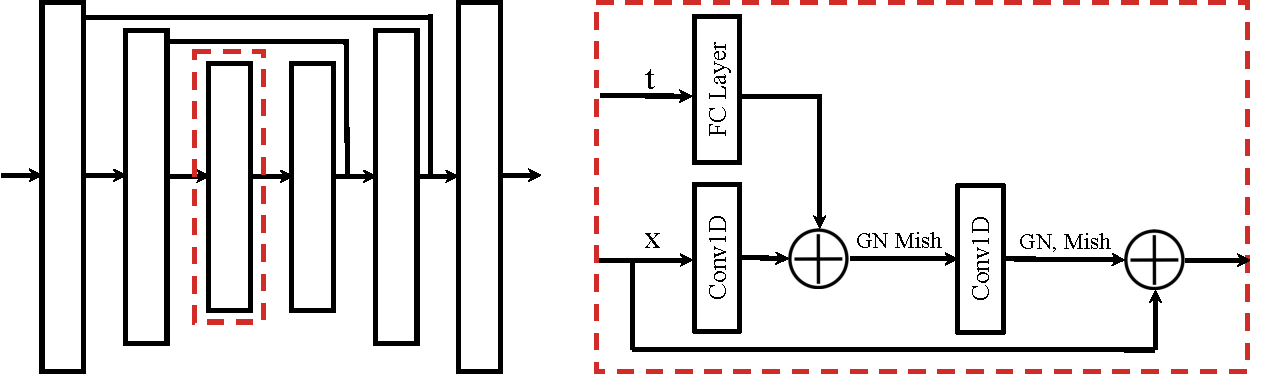
\includegraphics[width=\columnwidth]{images/architecture_v5.pdf}
\caption{
    \method has a U-Net architecture with residual blocks consisting of temporal convolutions, group normalization, and Mish nonlinearities.
}
\label{fig:app_architecture}
\end{figure}



\section{Test-time Flexibility}
\label{app:stacking_costs}

To guide \method{} to stack blocks in specified configurations, we used two separate perturbation functions $h(\btau{})$ to specify a given stack of block A on top of block B, which we detail below.

\myparagraph{Final State Matching} To enforce a final state consisting of block A on top of block B, we trained a perturbation function $h_{\text{match}}(\btau{})$ as a per-timestep classifier determining whether a a state $\vs$ exhibits a stack of block A on top of block B. We train the classifier on the demonstration data as the diffusion model.

\myparagraph{Contact Constraint} To guide the Kuka arm to stack block A on top of block B, we construct a perturbation function $h_{\text{contact}}(\btau{}) = \sum_{i=0}^{64} -1 * \|\btau{}_{c_i} - 1\|^2$, where $\btau{}_{c_i}$ corresponds to the underlying dimension in state $\btau{}_{s_i}$ that specifies the presence or absence of contact between the Kuka arm and block A.  We apply the contact constraint between the Kuka arm and block A for the first 64 timesteps in a trajectory, corresponding to initial contact with block A in a plan.


% \section{Cosine schedule for $\beta$ parameter}

\section{Implementation Details}

In this section we describe the architecture and record hyperparameters.

\begin{enumerate}
    \item The architecture of Diffuser (Figure~\ref{fig:app_architecture}) consists of a U-Net structure with 6 repeated residual blocks. Each block consisted of two temporal convolutions, each followed by group norm \citep{wu2018groupnorm}, and a final Mish nonlinearity \citep{misra2019mish}.
    Timestep embeddings are produced by a single fully-connected layer and added to the activations of the first temporal convolution within each block.
    \item We train the model using the Adam optimizer \citep{ba2015adam} with a learning rate of $4\mathrm{e}{-05}$ and batch size of $32$.
    We train the models for 500k steps.
    \item The return predictor $\mathcal{J}$ has the structure of the first half of the U-Net used for the diffusion model, with a final linear layer to produce a scalar output.
    \item We use a planning horizon $T$ of 32 in all locomotion tasks, $128$ for block-stacking, $128$ in \texttt{Maze2D / Multi2D U-Maze}, 265 in \texttt{Maze2D / Multi2D Medium}, and 384 in \texttt{Maze2D / Multi2D Large}.
    \item We found that we could reduce the planning horizon for many tasks, but that the guide scale would need to be lowered (\emph{e.g.}, to 0.001 for a horizon of $4$ in the \texttt{halfcheetah} tasks) to accommodate.
    The \href{https://github.com/jannerm/diffuser/blob/34d0e93296c6d8649187e6790ee41cf0c59e3631/config/locomotion.py#L163-L178}{configuration file} in the open-source code demonstrates how to run with a modified scale and horizon.
    \item We use $N=20$ diffusion steps for locomotion tasks and $N=100$ for block-stacking.
    \item We use a guide scale of $\alpha=0.1$ for all tasks except \texttt{hopper-medium-expert}, in which we use a smaller scale of $0.0001$.
    \item We used a discount factor of $0.997$ for the return prediction $\mathcal{J}_\phi$, though found that above $\gamma=0.99$ planning was fairly insensitive to changes in discount factor.
    \item We found that control performance was not substantially affected by the choice of predicting noise $\epsilon$ versus uncorrupted data $\btau{0}$ with the diffusion model.
\end{enumerate}

\end{appendices}